% Created 2024-09-24 Tue 13:24
% Intended LaTeX compiler: pdflatex
\documentclass[11pt]{article}
\usepackage[utf8]{inputenc}
\usepackage[T1]{fontenc}
\usepackage{graphicx}
\usepackage{longtable}
\usepackage{wrapfig}
\usepackage{rotating}
\usepackage[normalem]{ulem}
\usepackage{amsmath}
\usepackage{amssymb}
\usepackage{capt-of}
\usepackage{hyperref}
\author{Rumen Mitov}
\date{\today}
\title{Assignment 3}
\hypersetup{
 pdfauthor={Rumen Mitov},
 pdftitle={Assignment 3},
 pdfkeywords={},
 pdfsubject={},
 pdfcreator={Emacs 29.4 (Org mode 9.6.15)}, 
 pdflang={English}}
\begin{document}

\maketitle
\tableofcontents


\section{Problem 3.1}
\label{sec:org4627d90}
\uline{Search Interval}: [1, 1000000]

\subsection{Initial Hypothesis}
\label{sec:orgb65aee5}
I expect the execution time of the program to dacay exponentially as more threads are added up to a certain point. After this point I expect the execution time to rise slightly as the time taken to create more threads outweighs the time saved by those new threads.

\subsection{Results}
\label{sec:orga5f23fc}
\begin{center}
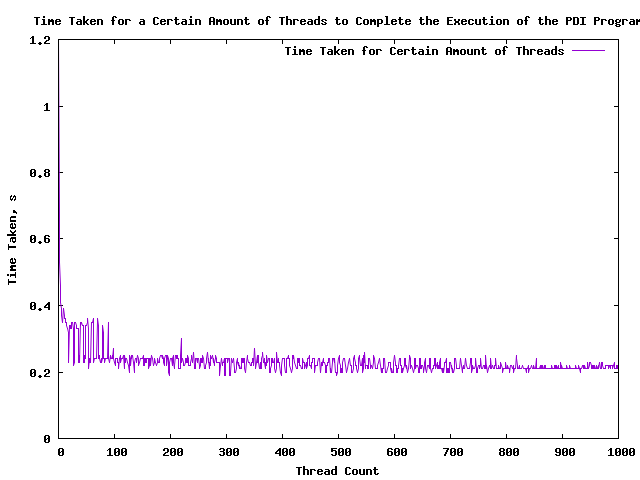
\includegraphics[width=.9\linewidth]{./assets/output.png}
\end{center}

As the graph above indicates the execution of the PDI program does indeed decay exponentially. After around 800 threads the gains of more threads seem minimal. This could be due to the fact that it takes time to spawn in new threads.

Additionally, the time recorded was real time, so there could be scheduler interupts pausing the execution of the program, which is another reason that the time does not drop beneath the 0.2s mark.

Finally, it would seem that my hypothesis that the extra threads would deteriorate the execution time to the extent that they actually cause the program to slow down, are incorrect.
\end{document}
